
\section{Stratification in {\large{\bf\slang}}}

%%\paa{notes}

%%this section has become cluttered, but for me the main results are the following:

%%\begin{enumerate}
%%\item Negation-, aggregation- and choice-free \lang programs have a unique minimal model (pure Datalog)
%%\item stratifiable \lang programs have a unique minimal model (again, Datalog, but we need to show that the restrictions and syntactic transformations
%%cannot introduce a cycle or add a negative edge to an existing cycle.)
%%\item \emph{temporally stratified} \lang programs (w/o choice) force any cycles with negation to involve an inductive edge, forcing an ordering on the evaluation.
%%we can show that in all such cases, the corresponding datalog program is modularly stratified (insofar as \emph{successor} is considered to be ``completely
%%evaluated" in a lower module.)  since modularly stratified programs have a unique stable model, so do any temporally stratified \lang programs.
%%\end{enumerate}

\begin{lemma} 
%
A \slang program without negation 
%%and aggregation 
has a unique
minimal model.
%
\end{lemma}

\begin{proof} 
%
A \slang program without negation 
%%and aggregation 
is a pure Datalog
program.  Every pure Datalog program has a unique minimal model. 
%
\end{proof}

%%\jmh{Oops, you forgot that this model is countably infinite due to infinite time. So I could add countably many random consistent facts and have an equally ``small'' model. You will need a more refined definition of safety and minimality that accounts for time.}

%%\jmh{I'm going to stop commenting here since you'll need some more machinery to continue.}

We define syntactic stratification of a \slang program the same way it is
defined for a Datalog program:

\begin{definition}
%
A \slang is \emph{syntactically stratifiable} if there
exists no cycle with a negative edge 
%%or an aggregation edge 
in the program's
predicate dependency graph.
%
\end{definition}

%%We evaluate such a program by evaluating each strongly connected component of
%%its predicate dependency graph under a closed-world assumption.  

We may evaluate such a program in any order returned by a topological sort on
the predicate dependency graph, with each strongly connected component
collapsed to a single node.

Since our translation from \slang to Datalog does not introduce any cycles or
negation to a program, a syntactically stratified \slang instance has a
unique minimal model, as any Datalog instance without choice has a unique
minimal model. 

%\begin{lemma}
%
%A syntactically stratifiable \lang instance without choice has a unique
%minimal model.  That is, there exists a function $D$ from syntactically
%stratifiable \lang instances without choice to their minimal models.
%
%\end{lemma}

%\begin{proof}
%\wrm{todo: insert statement that this is obvious}
%
%We know that there exists a function $B$ from syntactically stratifiable
%Datalog instances to their minimal models \wrm{cite?}.  Earlier, we introduced
%\wrm{XXX: where?} a bijection \wrm{XXX: probably not a bijection} $A$ from the
%set of \lang instances without choice to the set of Datalog instances, and a
%bijection $C$ between minimal models of Datalog instances and minimal models of
%\lang instances without choice.  We will show that $D = C \circ B \circ A$.

%Thus, we need only prove that the restriction of $A$ to syntactically
%stratifiable \lang instances without choice maps to a subset of syntactically
%stratifiable Datalog instances.  But this is clear, as $A$ does not add any
%rules to the instance, and may introduce only the non-negated EDB {\em
%successor} relation to the body of an existing rule.  Thus, $A$ cannot
%introduce any new cycle or add negation to any existing cycle in the instance's
%predicate dependency graph.
%
%\end{proof}

However, many programs we are interested in expressing are not syntactically
stratifiable.  Fortunately, \slang has a syntactically checkable notion of
{\em temporal stratifiability} that maps to a subset of {\em modularly
stratifiable}~\cite{modular} Datalog programs.

Intuitively, a Datalog instance is modularly stratifiable if no EDB
element depends negatively on itself.

%%\begin{example}
%%Consider a predicate \emph{print} that corresponds to a print queue.  The program below
%%states that if there is a message \{A, B\}, then there 
%%\begin{Dedalus}
%%print(A, B) \(\leftarrow\)
%%  message(A, B),
%%  \(\lnot\)print(A, B);
%%\end{Dedalus}
%%\end{example}

%Peter said we might not need these formal definitions.  Experimenting without
%\begin{definition}
%
%A Datalog program and EDB is \emph{locally stratifiable} if, after
%instantiating the rules given the Herbrand saturation of the program and EDB,
%there exists no cycle with a negation or aggregation edge in the dependency
%graph of instantiated ground atoms.
%
%\end{definition}

%We take the definition below from Ross~\cite{modular, ross-syntactic}.
%\begin{definition}
%
%A Datalog instance is \emph{modularly stratifiable} if, and only if its
%mutally recursive components are locally stratified once all instantiated rules
%with a false subgoal that is defined in a ``lower" component are removed.
%\end{definition}

%\begin{lemma}
%
%A locally stratifiable \lang instance without choice has a unique
%minimal model.  That is, there exists a function $E$ from locally
%stratifiable \lang instances without choice to their minimal models.
%
%\end{lemma}

%\begin{proof}
%
%\wrm{TODO}
%
%\end{proof}


\begin{definition}
%
The \emph{deductive reduction} of a \slang program $P$ is the subset of $P$
consisting of exactly those deductive rules in $P$.
%
\end{definition}

\begin{definition} 
%
A \slang program is \emph{temporally stratifiable} if its deductive
reduction is syntactically stratifiable.
%
\end{definition}

%%\newtheorem{theorem}{Theorem}
\begin{lemma}
%
Any temporally stratifiable \slang instance $P$ has a unique minimal model.
%
\end{lemma} 

\begin{proof}
%
{\bf Case 1:} $P$ consists of only deductive rules.  In this case, $P$'s
deductive reduction is $P$ itself.  We know $P$ is syntactically stratifiable,
thus it has a unique minimal model.

{\bf Case 2:} $P$ consists of both deductive and inductive rules.
Assume that $P$ does not have a unique minimal model.  This implies that $P$ is
not syntactically stratifiable.  Thus, there must exist some cycle through at
least one predicate $q$ involving negation.
%%or aggregation.  
Furthermore, this
cycle must involve an inductive rule, as $P$ is temporally stratified.

We convert our \slang program to a Datalog program $P'$ using the
transformation from Section~\ref{sec:abbrvsyntax}, which does not introduce
any additional cycles or negation.  Since the time suffix in the head of an
inductive rule is strictly greater than the time suffix of its body, no atom
may depend negatively on itself -- it may only depend negatively on atoms
in the previous timestep.  Thus, $P'$ is modularly stratified over time.
%
%does not have a unique minimal model.  This implies that $P$ is not
%syntactically stratifiable, thus there must exist some cycle through at least
%one predicate $q$ involving a negation or aggregation edge in $P$'s predicate
%dependency graph, and furthermore this cycle must include at least one
%inductive rule.  Since an inductive rule has a time suffix $S := N+1$, where
%$N$ is the timestamp of its body, and $P$'s deductive reduction is
%syntactically stratifiable, we know that the aggregate or negation of $q$
%must always occur in a strictly earlier or later timestamp than that of the
%positive $q$ atom.  Since the timestep in the cycle increases monotonically
%with each iteration, $q$ will never, in practice, depend on a negation or
%aggregate of itself.  Thus, $P$ is locally stratifiable, and by Lemma XXX
%above, $P$ has a unique minimal model.  This contradicts our assumption that
%$P$ does not have a unique minimal model.  Thus, $P$ has a unique minimal
%model.
%
\end{proof}


\begin{example}
A simple temporally stratifiable \slang program that is not syntactically stratifiable.

\begin{Dedalus}
r1
p(A, B, T)@next \(\leftarrow\)
  p(A, B, T),
  \(\lnot\)p_neg(A, B, T);
  
r2
p(A, B, T) \(\leftarrow\)
  insert\_p(A, B, T);

r3  
p_neg(A, B, T) \(\leftarrow\)
  p(A, B, T),
  delete\_p(T);
\end{Dedalus}

In the \slang program above, \emph{insert\_p} and \emph{delete\_p} are external events.
This reasonable program is unstratifiable because $p \succ del\_p \land del\_p \succ p$.  But because the successor relation is constrained
such that $\forall A,B (successor(A, B) \rightarrow B > A)$, any such program is modularly stratified on \emph{successor} 
Informally, we have $p_{n+1} \succ del\_p_{n} \succ p_{n}$.
\paa{need to make the text better, but this old example probably makes sense here}
\end{example}

\begin{figure}[t]
  \centering
  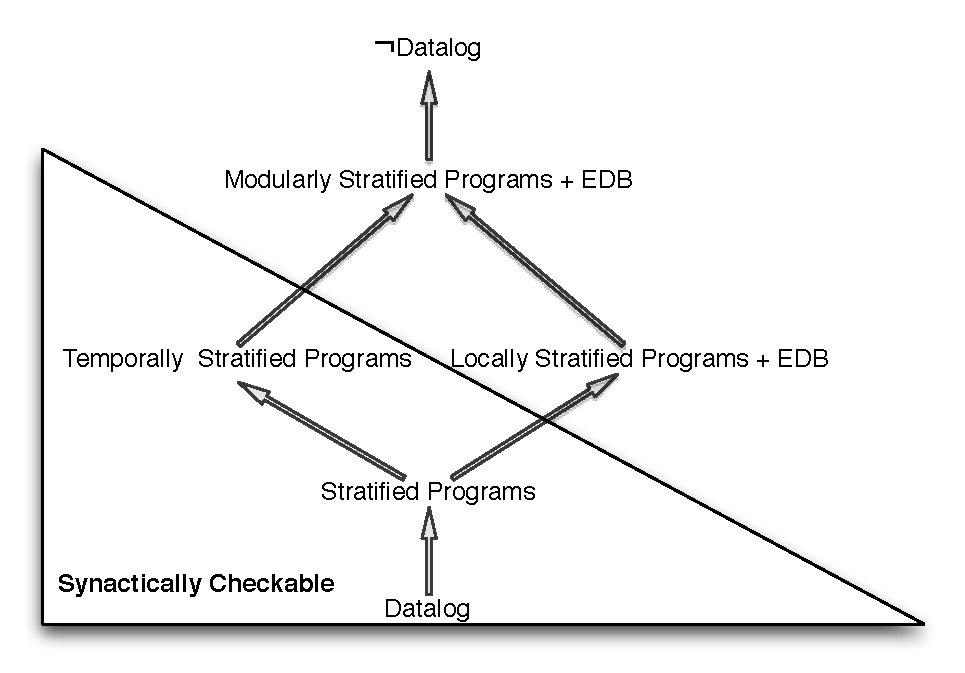
\includegraphics[width=0.75\linewidth]{figures/dedalus_classes.pdf}
  \label{fig:dedalus-classes}
  \caption{Stratifiablility classes.  $A \to B$ means that every program in A is in B.}
\vspace{-8pt}
\end{figure}


%%\paa{I don't think we can show that programs with async rules are locally stratifiable, actually}
%%\wrm{Why not?  What if we have that "causality constraint" we were talking about?}

